\section{Alloy}
	This section is intended to present a model of the system and his constraints using the Alloy modeling language. We have divided the Alloy code in four main sections:
		\begin{itemize}
			\item Signatures, here are modeled the entities of our system. In the firs part there are primitive entities like boolean or strings and in the second part there are the system entities.
			\item Facts, here are modeled all the constraints for our model.
			\item Predicates and Assertions, here are modeled all the checks to control the consinstency of our model.
			\item Generated World, here there is an example of entities of our system generated by the "show" predicate in the Predicates and Assertions section.
		\end{itemize}

		\subsection{Signatures}
		Here there are attached screenshots of the Alloy code about entities:

				\begin{figure}[H]
					\centering
					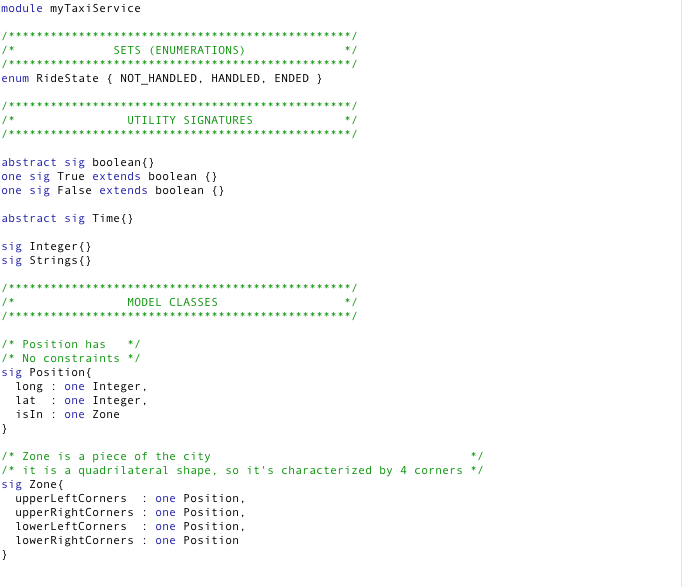
\includegraphics[width=\textwidth, scale=0.5]{IMG/ALLOY/SIG_1.png}
					\caption{Signatures 1}\label{sec:FigureSignatures1}
				\end{figure}

				\begin{figure}[H]
					\centering
					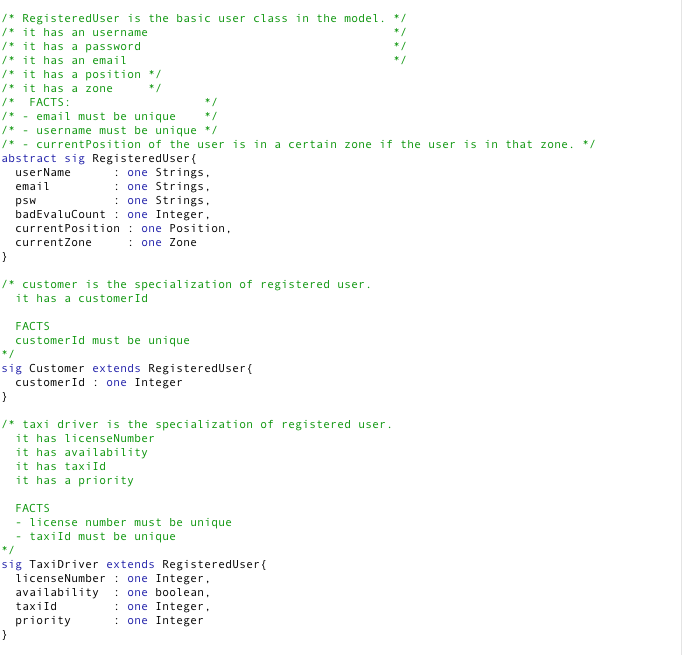
\includegraphics[width=\textwidth, scale=0.5]{IMG/ALLOY/SIG_2.png}
					\caption{Signatures 2}\label{sec:FigureSignatures2}
				\end{figure}

				\begin{figure}[H]
					\centering
					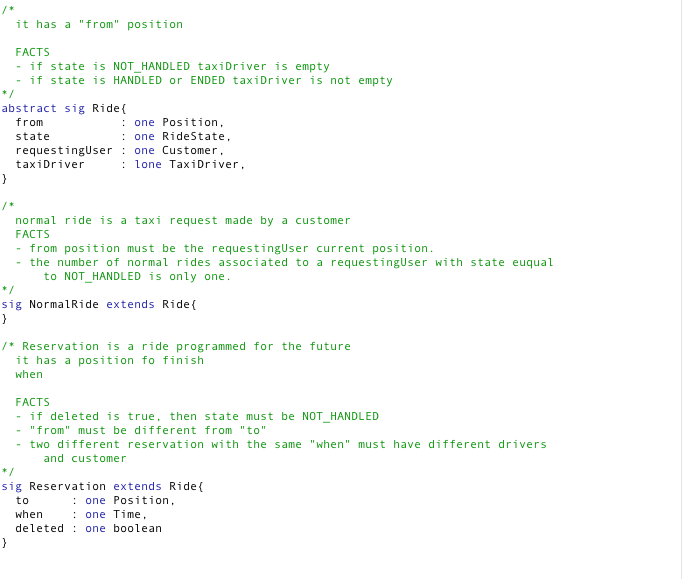
\includegraphics[width=\textwidth, scale=0.5]{IMG/ALLOY/SIG_3.png}
					\caption{Signatures 3}\label{sec:FigureSignatures3}
				\end{figure}

		\subsection{Facts}
		Here there are attached screenshots of the Alloy code about rules:

				\begin{figure}[H]
					\centering
					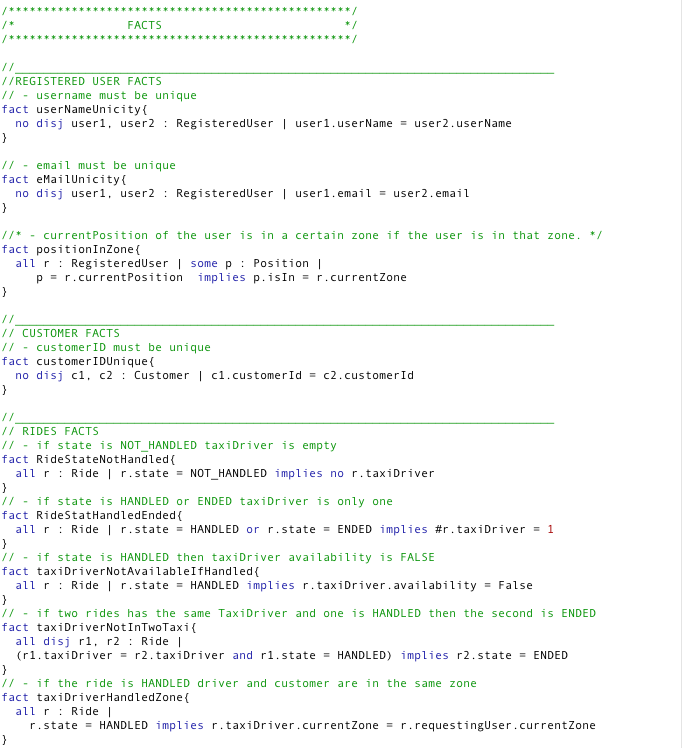
\includegraphics[width=\textwidth, scale=0.5]{IMG/ALLOY/FACT_1.png}
					\caption{Facts 1}\label{sec:FigureFacts1}
				\end{figure}

				\begin{figure}[H]
					\centering
					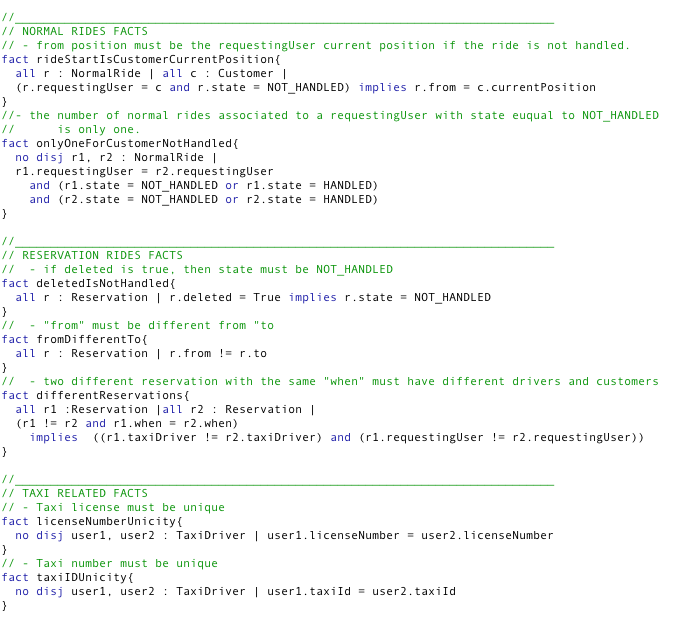
\includegraphics[width=\textwidth, scale=0.5]{IMG/ALLOY/FACT_2.png}
					\caption{Facts 2}\label{sec:FigureFacts2}
				\end{figure}

		\subsection{Predicates and Assertions}
		Here there are attached screenshots of the Alloy code about checks:

				\begin{figure}[H]
					\centering
					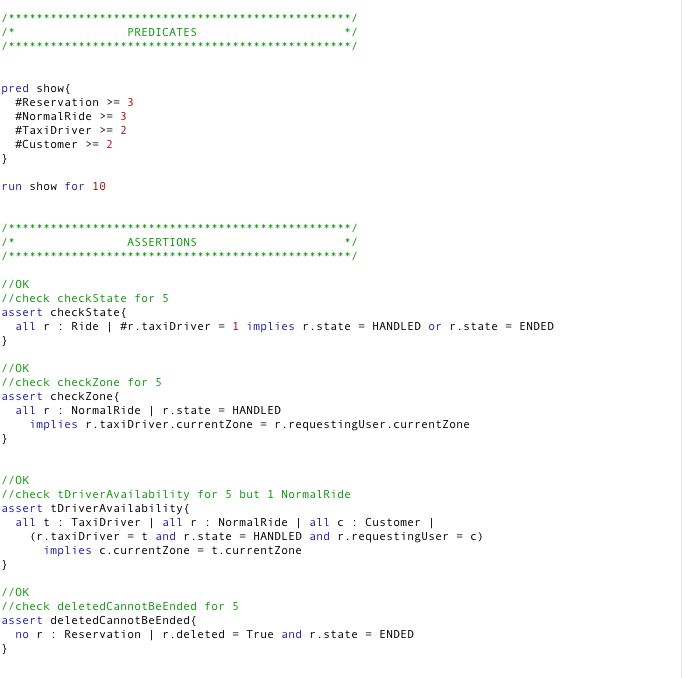
\includegraphics[width=\textwidth, scale=0.5]{IMG/ALLOY/PREN_ASS.png}
					\caption{Predicates and Assertions 1}\label{sec:FigureSignatures1}
				\end{figure}

		\subsection{Generated World}
		Here is the attached a screenshot of the entities generated by the "show" predicate:

				\begin{figure}[H]
					\centering
					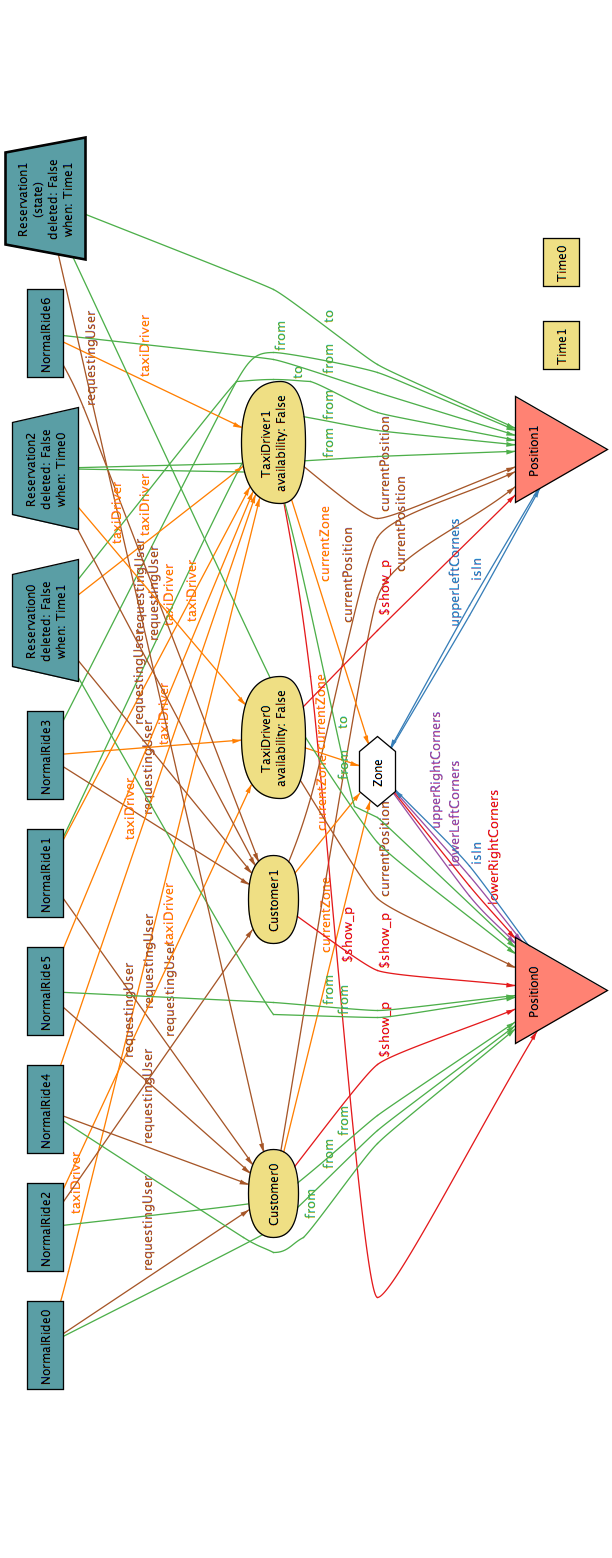
\includegraphics[width=\textwidth, height=\textheight, scale=0.5]{IMG/ALLOY/alloyWorld.png}
					\caption{Alloy World 1}\label{sec:FigureAlloyWorld1}
				\end{figure}		